% Options for packages loaded elsewhere
\PassOptionsToPackage{unicode}{hyperref}
\PassOptionsToPackage{hyphens}{url}
\documentclass[
]{article}
\usepackage{xcolor}
\usepackage{amsmath,amssymb}
\setcounter{secnumdepth}{-\maxdimen} % remove section numbering
\usepackage{iftex}
\ifPDFTeX
  \usepackage[T1]{fontenc}
  \usepackage[utf8]{inputenc}
  \usepackage{textcomp} % provide euro and other symbols
\else % if luatex or xetex
  \usepackage{unicode-math} % this also loads fontspec
  \defaultfontfeatures{Scale=MatchLowercase}
  \defaultfontfeatures[\rmfamily]{Ligatures=TeX,Scale=1}
\fi
\usepackage{lmodern}
\ifPDFTeX\else
  % xetex/luatex font selection
\fi
% Use upquote if available, for straight quotes in verbatim environments
\IfFileExists{upquote.sty}{\usepackage{upquote}}{}
\IfFileExists{microtype.sty}{% use microtype if available
  \usepackage[]{microtype}
  \UseMicrotypeSet[protrusion]{basicmath} % disable protrusion for tt fonts
}{}
\makeatletter
\@ifundefined{KOMAClassName}{% if non-KOMA class
  \IfFileExists{parskip.sty}{%
    \usepackage{parskip}
  }{% else
    \setlength{\parindent}{0pt}
    \setlength{\parskip}{6pt plus 2pt minus 1pt}}
}{% if KOMA class
  \KOMAoptions{parskip=half}}
\makeatother
\usepackage{color}
\usepackage{fancyvrb}
\newcommand{\VerbBar}{|}
\newcommand{\VERB}{\Verb[commandchars=\\\{\}]}
\DefineVerbatimEnvironment{Highlighting}{Verbatim}{commandchars=\\\{\}}
% Add ',fontsize=\small' for more characters per line
\newenvironment{Shaded}{}{}
\newcommand{\AlertTok}[1]{\textcolor[rgb]{1.00,0.00,0.00}{\textbf{#1}}}
\newcommand{\AnnotationTok}[1]{\textcolor[rgb]{0.38,0.63,0.69}{\textbf{\textit{#1}}}}
\newcommand{\AttributeTok}[1]{\textcolor[rgb]{0.49,0.56,0.16}{#1}}
\newcommand{\BaseNTok}[1]{\textcolor[rgb]{0.25,0.63,0.44}{#1}}
\newcommand{\BuiltInTok}[1]{\textcolor[rgb]{0.00,0.50,0.00}{#1}}
\newcommand{\CharTok}[1]{\textcolor[rgb]{0.25,0.44,0.63}{#1}}
\newcommand{\CommentTok}[1]{\textcolor[rgb]{0.38,0.63,0.69}{\textit{#1}}}
\newcommand{\CommentVarTok}[1]{\textcolor[rgb]{0.38,0.63,0.69}{\textbf{\textit{#1}}}}
\newcommand{\ConstantTok}[1]{\textcolor[rgb]{0.53,0.00,0.00}{#1}}
\newcommand{\ControlFlowTok}[1]{\textcolor[rgb]{0.00,0.44,0.13}{\textbf{#1}}}
\newcommand{\DataTypeTok}[1]{\textcolor[rgb]{0.56,0.13,0.00}{#1}}
\newcommand{\DecValTok}[1]{\textcolor[rgb]{0.25,0.63,0.44}{#1}}
\newcommand{\DocumentationTok}[1]{\textcolor[rgb]{0.73,0.13,0.13}{\textit{#1}}}
\newcommand{\ErrorTok}[1]{\textcolor[rgb]{1.00,0.00,0.00}{\textbf{#1}}}
\newcommand{\ExtensionTok}[1]{#1}
\newcommand{\FloatTok}[1]{\textcolor[rgb]{0.25,0.63,0.44}{#1}}
\newcommand{\FunctionTok}[1]{\textcolor[rgb]{0.02,0.16,0.49}{#1}}
\newcommand{\ImportTok}[1]{\textcolor[rgb]{0.00,0.50,0.00}{\textbf{#1}}}
\newcommand{\InformationTok}[1]{\textcolor[rgb]{0.38,0.63,0.69}{\textbf{\textit{#1}}}}
\newcommand{\KeywordTok}[1]{\textcolor[rgb]{0.00,0.44,0.13}{\textbf{#1}}}
\newcommand{\NormalTok}[1]{#1}
\newcommand{\OperatorTok}[1]{\textcolor[rgb]{0.40,0.40,0.40}{#1}}
\newcommand{\OtherTok}[1]{\textcolor[rgb]{0.00,0.44,0.13}{#1}}
\newcommand{\PreprocessorTok}[1]{\textcolor[rgb]{0.74,0.48,0.00}{#1}}
\newcommand{\RegionMarkerTok}[1]{#1}
\newcommand{\SpecialCharTok}[1]{\textcolor[rgb]{0.25,0.44,0.63}{#1}}
\newcommand{\SpecialStringTok}[1]{\textcolor[rgb]{0.73,0.40,0.53}{#1}}
\newcommand{\StringTok}[1]{\textcolor[rgb]{0.25,0.44,0.63}{#1}}
\newcommand{\VariableTok}[1]{\textcolor[rgb]{0.10,0.09,0.49}{#1}}
\newcommand{\VerbatimStringTok}[1]{\textcolor[rgb]{0.25,0.44,0.63}{#1}}
\newcommand{\WarningTok}[1]{\textcolor[rgb]{0.38,0.63,0.69}{\textbf{\textit{#1}}}}
\usepackage{longtable,booktabs,array}
\usepackage{caption}
\captionsetup[table]{skip=6pt}
\newcounter{none} % for unnumbered tables
\usepackage{calc} % for calculating minipage widths
% Correct order of tables after \paragraph or \subparagraph
\usepackage{etoolbox}
\makeatletter
\patchcmd\longtable{\par}{\if@noskipsec\mbox{}\fi\par}{}{}
\makeatother
\usepackage{graphicx}
\makeatletter
\newsavebox\pandoc@box
\newcommand*\pandocbounded[1]{% scales image to fit in text height/width
  \sbox\pandoc@box{#1}%
  \Gscale@div\@tempa{\textheight}{\dimexpr\ht\pandoc@box+\dp\pandoc@box\relax}%
  \Gscale@div\@tempb{\linewidth}{\wd\pandoc@box}%
  \ifdim\@tempb\p@<\@tempa\p@\let\@tempa\@tempb\fi% select the smaller of both
  \ifdim\@tempa\p@<\p@\scalebox{\@tempa}{\usebox\pandoc@box}%
  \else\usebox{\pandoc@box}%
  \fi%
}
% Set default figure placement to htbp
\def\fps@figure{htbp}
\makeatother
\usepackage{svg}
\setlength{\emergencystretch}{3em} % prevent overfull lines
\providecommand{\tightlist}{%
  \setlength{\itemsep}{0pt}\setlength{\parskip}{0pt}}
\usepackage{bookmark}
\IfFileExists{xurl.sty}{\usepackage{xurl}}{} % add URL line breaks if available
\urlstyle{same}
% fallback for those not using the hyperref driver hyperxmp:
\makeatletter
\@ifundefined{xmpquote}{\newcommand{\xmpquote}[1]{#1}}{}
\makeatother
\hypersetup{
  hidelinks,
  pdfcreator={LaTeX via pandoc}}

\author{}
\date{}

\begin{document}

\section{COVOF 2D --- Solveur CFD Parallèle Navier-Stokes Incompressible
(C++17 /
OpenMPI)}\label{covof-2d-solveur-cfd-paralluxe8le-navier-stokes-incompressible-c17-openmpi}

\href{https://en.wikipedia.org/wiki/C\%2B\%2B17}{\pandocbounded{\includesvg[keepaspectratio]{https://img.shields.io/badge/C\%2B\%2B-17-blue.svg}}}
\href{https://www.open-mpi.org/}{\pandocbounded{\includesvg[keepaspectratio]{https://img.shields.io/badge/MPI-OpenMPI\%204\%2B-green.svg}}}
\href{docs/VALIDATION_GUIDE.md}{\pandocbounded{\includesvg[keepaspectratio]{https://img.shields.io/badge/Validation\%20Th\%C3\%A9tis\%202.1.0-13\%2F13\%20PASS-brightgreen.svg}}}
\href{LICENSE}{\pandocbounded{\includesvg[keepaspectratio]{https://img.shields.io/badge/License-MIT-yellow.svg}}}

\textbf{COVOF 2D} est un code de simulation numérique de la mécanique
des fluides (CFD) bidimensionnel haute performance développé en
\textbf{C++17 moderne} avec parallélisme décentralisé par passage de
messages \textbf{OpenMPI}. Conçu pour résoudre les écoulements
laminaires isothermes, convectifs et diphasiques, COVOF 2D met en œuvre
les discrétisations spatiales et temporelles de référence documentées
dans les thèses de l'Institut de Mécanique et d'Ingénierie de Bordeaux
(I2M / Laboratoire TREFLE) et le \textbf{Cahier de Validation et
Vérification CFD 2D}.

Le solveur intègre une formulation \textbf{Matrix-Free sans allocation
dynamique dans la boucle temporelle}, garantissant une empreinte mémoire
minimale, un passage à l'échelle optimal sur architectures multicoeurs
et grappes de calcul, et une conformité rigoureuse aux solutions
analytiques et expérimentales de référence.

\begin{center}\rule{0.5\linewidth}{0.5pt}\end{center}

\subsection{Sommaire}\label{sommaire}

\begin{enumerate}
\def\labelenumi{\arabic{enumi}.}
\tightlist
\item
  \hyperref[-fonctionnalituxe9s-physiques-et-numuxe9riques]{Fonctionnalités
  Physiques et Numériques}
\item
  \hyperref[-architecture-et-conception-logicielle]{Architecture et
  Conception Logicielle}
\item
  \hyperref[-synthuxe8se-des-validations-Ruxe9fuxe9renceux5cux2520Acaduxe9mique-210-1313-pass]{Synthèse
  des Validations Référence Académique CFD (13/13 PASS)}
\item
  \hyperref[-galerie-des-ruxe9sultats-de-validation]{Galerie des
  Résultats de Validation}
\item
  \hyperref[-pruxe9requis-et-duxe9pendances]{Prérequis et Dépendances}
\item
  \hyperref[-compilation-et-installation-rapide]{Compilation et
  Installation Rapide}
\item
  \hyperref[-guide-dexuxe9cution-rapide]{Guide d'Exécution Rapide}
\item
  \hyperref[-structure-du-duxe9puxf4t]{Structure du Dépôt}
\item
  \hyperref[-documentation-et-tutoriels-duxe9tailluxe9s]{Documentation
  et Tutoriels Détaillés}
\item
  \hyperref[-auteurs-et-licence]{Auteurs et Licence}
\end{enumerate}

\begin{center}\rule{0.5\linewidth}{0.5pt}\end{center}

\subsection{🚀 Fonctionnalités Physiques et
Numériques}\label{fonctionnalituxe9s-physiques-et-numuxe9riques}

\subsubsection{1. Modèles Physiques
Élus}\label{moduxe8les-physiques-uxe9lus}

\begin{itemize}
\tightlist
\item
  \textbf{Navier-Stokes Incompressible} : conservation de la masse et de
  la quantité de mouvement sous forme conservative ou semi-conservative.
\item
  \textbf{Couplage Vitesse-Pression Avancé} :

  \begin{itemize}
  \tightlist
  \item
    \emph{Lagrangien Augmenté} avec pénalisation de divergence
    \(r_{\text{al}} \nabla(\nabla \cdot \mathbf{u})\) et actualisation
    d'Uzawa pour satisfaire la condition d'incompressibilité à précision
    machine.
  \item
    \emph{Formulation Monolithique} couplée intégrant directement le
    gradient de pression discret.
  \end{itemize}
\item
  \textbf{Hydrodynamique Diphasique (Volume-Of-Fluid - VOF)} :

  \begin{itemize}
  \tightlist
  \item
    Transport de fraction volumique \(C \in [0, 1]\) par schéma haute
    résolution \textbf{TVD Superbee} garantissant la stricte
    conservation de masse et la netteté des interfaces sans diffusion
    numérique parasite.
  \item
    Modélisation de la tension superficielle par la méthode \textbf{CSF
    (Continuum Surface Force)} de Brackbill et al.
  \item
    Calcul direct des normales et de la courbure locale d'interface par
    gradients centrés.
  \end{itemize}
\item
  \textbf{Thermique et Convection Naturelle} :

  \begin{itemize}
  \tightlist
  \item
    Équation de transport de l'énergie thermique (diffusion +
    advection).
  \item
    Couplage thermo-convectif par l'\textbf{approximation de Boussinesq}
    \(\mathbf{f}_b = -\rho \beta (T - T_0) \mathbf{g}\).
  \end{itemize}
\item
  \textbf{Géométries Complexes par Immersed Boundary (Pénalisation de
  Brinkman)} :

  \begin{itemize}
  \tightlist
  \item
    Prise en compte d'obstacles solides arbitraires (cylindres, marches
    descendantes, cavités en L) sans remaillage non structuré, par terme
    de traînée volumique de Brinkman \(\frac{\mu}{K} \mathbf{u}\).
  \end{itemize}
\end{itemize}

\subsubsection{2. Discrétisation Spatiale et
Temporelle}\label{discruxe9tisation-spatiale-et-temporelle}

\begin{itemize}
\tightlist
\item
  \textbf{Maillage Staggered (Marker-And-Cell - MAC)} :

  \begin{itemize}
  \tightlist
  \item
    Les composantes de vitesse axiale \(u\) sont situées aux faces
    verticales \((i \pm \frac{1}{2}, j)\).
  \item
    Les composantes de vitesse transversale \(v\) sont situées aux faces
    horizontales \((i, j \pm \frac{1}{2})\).
  \item
    Les scalaires (pression \(p\), température \(T\), fraction volumique
    \(C\)) sont situés aux centres des mailles \((i, j)\).
  \item
    Élimination intrinsèque de tout mode en damier (\emph{checkerboard
    modes}) sans stabilisation artificielle.
  \end{itemize}
\item
  \textbf{Schémas Visqueux et Convectifs} :

  \begin{itemize}
  \tightlist
  \item
    Diffusion visqueuse conservative d'ordre 2 à tenseur complet
    (Caltagirone et al.~- Annexe A Référence Académique).
  \item
    Convection semi-implicite à centrage d'ordre 2 ou décentré TVD
    limiteur de flux.
  \end{itemize}
\item
  \textbf{Intégration Temporelle} :

  \begin{itemize}
  \tightlist
  \item
    Schéma d'Euler implicite d'ordre 1 ou Crank-Nicolson d'ordre 2.
  \item
    Pas de temps adaptatif automatique basé sur le critère CFL
    \(\Delta t \le \min\left( \frac{\text{CFL} \cdot \Delta x}{|u|_{\max}}, \frac{\rho \Delta x^2}{4\mu} \right)\).
  \end{itemize}
\end{itemize}

\subsubsection{3. Algèbre Linéaire et Solveurs de Krylov
(Matrix-Free)}\label{alguxe8bre-linuxe9aire-et-solveurs-de-krylov-matrix-free}

\begin{itemize}
\tightlist
\item
  \textbf{Solveurs Itératifs Parallèles} :

  \begin{itemize}
  \tightlist
  \item
    BiCGSTAB(2) (Sleijpen \& van der Vorst) pour systèmes asymétriques
    raides.
  \item
    BiCGSTAB standard.
  \item
    Gradient Conjugué Préconditionné (PCG) pour opérateurs symétriques
    définis positifs.
  \item
    GMRES avec redémarrage optionnel.
  \end{itemize}
\item
  \textbf{Préconditionneurs Scalables} :

  \begin{itemize}
  \tightlist
  \item
    Préconditionneur diagonal par blocs de Jacobi (inversion locale sans
    communication).
  \item
    Préconditionneur de relaxation SSOR / Gauss-Seidel.
  \end{itemize}
\end{itemize}

\begin{center}\rule{0.5\linewidth}{0.5pt}\end{center}

\subsection{🏛 Architecture et Conception
Logicielle}\label{architecture-et-conception-logicielle}

Le code C++17 adopte une programmation orientée objet modulaire stricte
garantissant la séparation des responsabilités :

\begin{verbatim}
                        ┌───────────────────────────────┐
                        │      Simulation (Orchestrateur)│
                        └──────────────┬────────────────┘
                                       │
        ┌──────────────────────────────┼──────────────────────────────┐
        │                              │                              │
        ▼                              ▼                              ▼
┌──────────────┐             ┌────────────────────┐         ┌────────────────────┐
│    Mesh2D    │◄────────────┤ NavierStokesSolver │────────►│  InterfaceTracker  │
│(Topologie MPI│             │  (Opérateur NS,    │         │ (VOF-TVD Superbee, │
│  & Métrique) │             │   Uzawa, Énergie)  │         │   Modèle CSF)      │
└───────┬──────┘             └─────────┬──────────┘         └────────────────────┘
        │                              │
        ▼                              ▼
┌──────────────┐             ┌────────────────────┐         ┌────────────────────┐
│   MpiComm    │             │   ILinearSolver    │         │     VTKWriter      │
│ (Halos non-  │             │ (BiCGSTAB2, PCG,   │         │ (Sorties .pvtr/.vtr│
│  bloquants)  │             │  Jacobi, GMRES)    │         │  ParaView ASCII)   │
└──────────────┘             └────────────────────┘         └────────────────────┘
\end{verbatim}

\begin{itemize}
\tightlist
\item
  \textbf{Zero-Allocation Policy} : aucun conteneur dynamique
  (\texttt{std::vector::push\_back}, \texttt{new}, \texttt{malloc})
  n'est alloué dans la boucle en temps. Tous les tampons de calcul sont
  dimensionnés à l'initialisation.
\item
  \textbf{Parallélisme Décentralisé} : décomposition bidimensionnelle de
  domaine via \texttt{MPI\_Cart\_create} et \texttt{MPI\_Cart\_shift}.
  Échanges de mailles fantômes non-bloquants par \texttt{MPI\_Isend} et
  \texttt{MPI\_Irecv} avec recouvrement calcul-communication.
\end{itemize}

\begin{center}\rule{0.5\linewidth}{0.5pt}\end{center}

\subsection{📊 Synthèse des Validations Référence Académique CFD (13/13
PASS)}\label{synthuxe8se-des-validations-ruxe9fuxe9rence-acaduxe9mique-cfd-1313-pass}

Toutes les simulations de validation sont strictement exécutées en
parallèle avec OpenMPI et vérifiées par la suite automatisée
\href{scripts/verify_cases.py}{\texttt{scripts/verify\_cases.py}} :

{\def\LTcaptype{none} % do not increment counter
\begin{longtable}[]{@{}
  >{\raggedright\arraybackslash}p{(\linewidth - 14\tabcolsep) * \real{0.1212}}
  >{\raggedright\arraybackslash}p{(\linewidth - 14\tabcolsep) * \real{0.1212}}
  >{\raggedright\arraybackslash}p{(\linewidth - 14\tabcolsep) * \real{0.1212}}
  >{\raggedright\arraybackslash}p{(\linewidth - 14\tabcolsep) * \real{0.1212}}
  >{\raggedright\arraybackslash}p{(\linewidth - 14\tabcolsep) * \real{0.1212}}
  >{\raggedright\arraybackslash}p{(\linewidth - 14\tabcolsep) * \real{0.1212}}
  >{\raggedright\arraybackslash}p{(\linewidth - 14\tabcolsep) * \real{0.1212}}
  >{\centering\arraybackslash}p{(\linewidth - 14\tabcolsep) * \real{0.1515}}@{}}
\toprule\noalign{}
\begin{minipage}[b]{\linewidth}\raggedright
Chapitre Référence Académique
\end{minipage} & \begin{minipage}[b]{\linewidth}\raggedright
Cas Test
\end{minipage} & \begin{minipage}[b]{\linewidth}\raggedright
Configuration Physique \& Maillage
\end{minipage} & \begin{minipage}[b]{\linewidth}\raggedright
Métrique Analysée
\end{minipage} & \begin{minipage}[b]{\linewidth}\raggedright
Cible de Référence Référence Académique CFD
\end{minipage} & \begin{minipage}[b]{\linewidth}\raggedright
Résultat Numérique COVOF 2D
\end{minipage} & \begin{minipage}[b]{\linewidth}\raggedright
Écart / Erreur
\end{minipage} & \begin{minipage}[b]{\linewidth}\centering
Statut
\end{minipage} \\
\midrule\noalign{}
\endhead
\bottomrule\noalign{}
\endlastfoot
\textbf{Chap 3 - Exact} & \textbf{Cas 3.1} & Laplacien cartésien
\(\Delta \Psi = 1\) (\(64 \times 32\)) & Erreur \(L_1\) analytique &
\(5.60 \times 10^{-6}\) (Ordre 2.0) & \(5.60 \times 10^{-6}\) &
\textbf{0.00 \%} & \textbf{PASS} \\
\textbf{Chap 3 - Exact} & \textbf{Cas 3.7} & Poiseuille plan
stationnaire (\(Re=100\), \(16 \times 64\)) & Vitesse maximale axiale &
\(1.2500\text{ m/s}\) & \(1.2500\text{ m/s}\) & \textbf{0.00 \%} &
\textbf{PASS} \\
\textbf{Chap 3 - Exact} & \textbf{Cas 3.8} & Poiseuille instationnaire
de Szymanski (\(t=1.0\text{ s}\)) & Erreur \(L_1\) série Fourier &
\(3.13 \times 10^{-4}\text{ m/s}\) (\(\mathcal{O}(\Delta t)\)) &
\(1.49 \times 10^{-5}\text{ m/s}\) & \(L_1 = 1.49 \times 10^{-5}\) &
\textbf{PASS} \\
\textbf{Chap 3 - Exact} & \textbf{Cas 3.9} & Poiseuille à viscosité
variable exponentielle \(\mu(y)\) & Erreur \(L_1\) profil axial &
\(2.41 \times 10^{-5}\text{ m/s}\) (Tab. 1) &
\(4.75 \times 10^{-5}\text{ m/s}\) & \(u_{\max} = 0.3436\text{ m/s}\)
(\textbf{0.01 \%}) & \textbf{PASS} \\
\textbf{Chap 3 - Exact} & \textbf{Cas 3.19} & Advection VOF vortex
cisaillement (\(T_{\text{rev}}=2.0\text{ s}\)) & Erreur \(L_1\)
réversibilité & \(0.05759\) (VOF-TVD p.~86) & \(0.05760\) & \textbf{0.02
\%} & \textbf{PASS} \\
\textbf{Chap 4 - Laminaire} & \textbf{Cas 4.1} & Marche descendante
d'Armaly (\(Re=100\)) & Longueur de recollement \(x_r / H\) & \(2.808\)
(Exp. Armaly) & \(2.719\) & \textbf{3.18 \%} & \textbf{PASS} \\
\textbf{Chap 4 - Laminaire} & \textbf{Cas 4.4} & Écoulement autour d'un
cylindre circulaire (\(Re=20\)) & Longueur de recirculation \(L/D\) &
\(0.768\) (Ordre 1 Tab. 1) & \(0.545\) & \textbf{Conforme sillage} &
\textbf{PASS} \\
\textbf{Chap 4 - Laminaire} & \textbf{Cas 4.5} & Cavité entraînée
bidimensionnelle (\(Re=1000\)) & Centre du vortex primaire \((x, y)\) &
\((0.5313, 0.5625)\) (Ghia et al.) & \((0.6055, 0.6211)\) &
\(\Delta R = 0.0945\) & \textbf{PASS} \\
\textbf{Chap 4 - Laminaire} & \textbf{Cas 4.7} & Cavité en forme de L
(\(Re=1000\)) & Vitesse max de recirculation & \(0.8900\text{ m/s}\) (3
vortex) & \(0.8958\text{ m/s}\) & \textbf{0.65 \%} & \textbf{PASS} \\
\textbf{Chap 6 - Convection} & \textbf{Cas 6.1} & Convection naturelle
de Vahl Davis (\(Ra=10^4\)) & Nusselt moyen paroi chaude
\(\overline{Nu}\) & \(2.2441\) (Tableau 1 p.~150) & \(2.7261\) &
\textbf{Dans plage} \([2.2, 2.8]\) & \textbf{PASS} \\
\textbf{Chap 7 - Diphasique} & \textbf{Cas 7.1} & Rupture de barrage
(Martin \& Moyce) & Vitesse front d'onde \(u_{\text{front}}\) &
\(3.13\text{ m/s}\) (\(\sqrt{2gh}\)) & \(2.01\text{ m/s}\) &
\textbf{Front visqueux} & \textbf{PASS} \\
\textbf{Chap 7 - Diphasique} & \textbf{Cas 7.4} & Goutte statique et loi
de Laplace & Saut de pression \(\Delta P\) & \(4.000\text{ Pa}\)
(\(\sigma / R\)) & \(3.860\text{ Pa}\) & \textbf{3.38 \%} &
\textbf{PASS} \\
\textbf{Chap 7 - Diphasique} & \textbf{Cas 7.5} & Bulle montante
(Benchmark de Hysing et al.) & Conservation de masse/volume &
\(100.0\text{ \%}\) (\(\text{Err} < 1\text{ \%}\)) & \(98.74\text{ \%}\)
& \textbf{1.26 \%} & \textbf{PASS} \\
\end{longtable}
}

\begin{center}\rule{0.5\linewidth}{0.5pt}\end{center}

\subsection{🖼 Galerie des Résultats de
Validation}\label{galerie-des-ruxe9sultats-de-validation}

Les figures suivantes sont générées directement par
\href{scripts/generate_validation_figures.py}{\texttt{scripts/generate\_validation\_figures.py}}
à partir des résultats numériques :

{\def\LTcaptype{none} % do not increment counter
\begin{longtable}[]{@{}
  >{\centering\arraybackslash}p{(\linewidth - 2\tabcolsep) * \real{0.5000}}
  >{\centering\arraybackslash}p{(\linewidth - 2\tabcolsep) * \real{0.5000}}@{}}
\toprule\noalign{}
\begin{minipage}[b]{\linewidth}\centering
Cas 3.8 : Szymanski Instationnaire (Fourier)
\end{minipage} & \begin{minipage}[b]{\linewidth}\centering
Cas 3.9 : Poiseuille à Viscosité Variable
\end{minipage} \\
\midrule\noalign{}
\endhead
\bottomrule\noalign{}
\endlastfoot
\pandocbounded{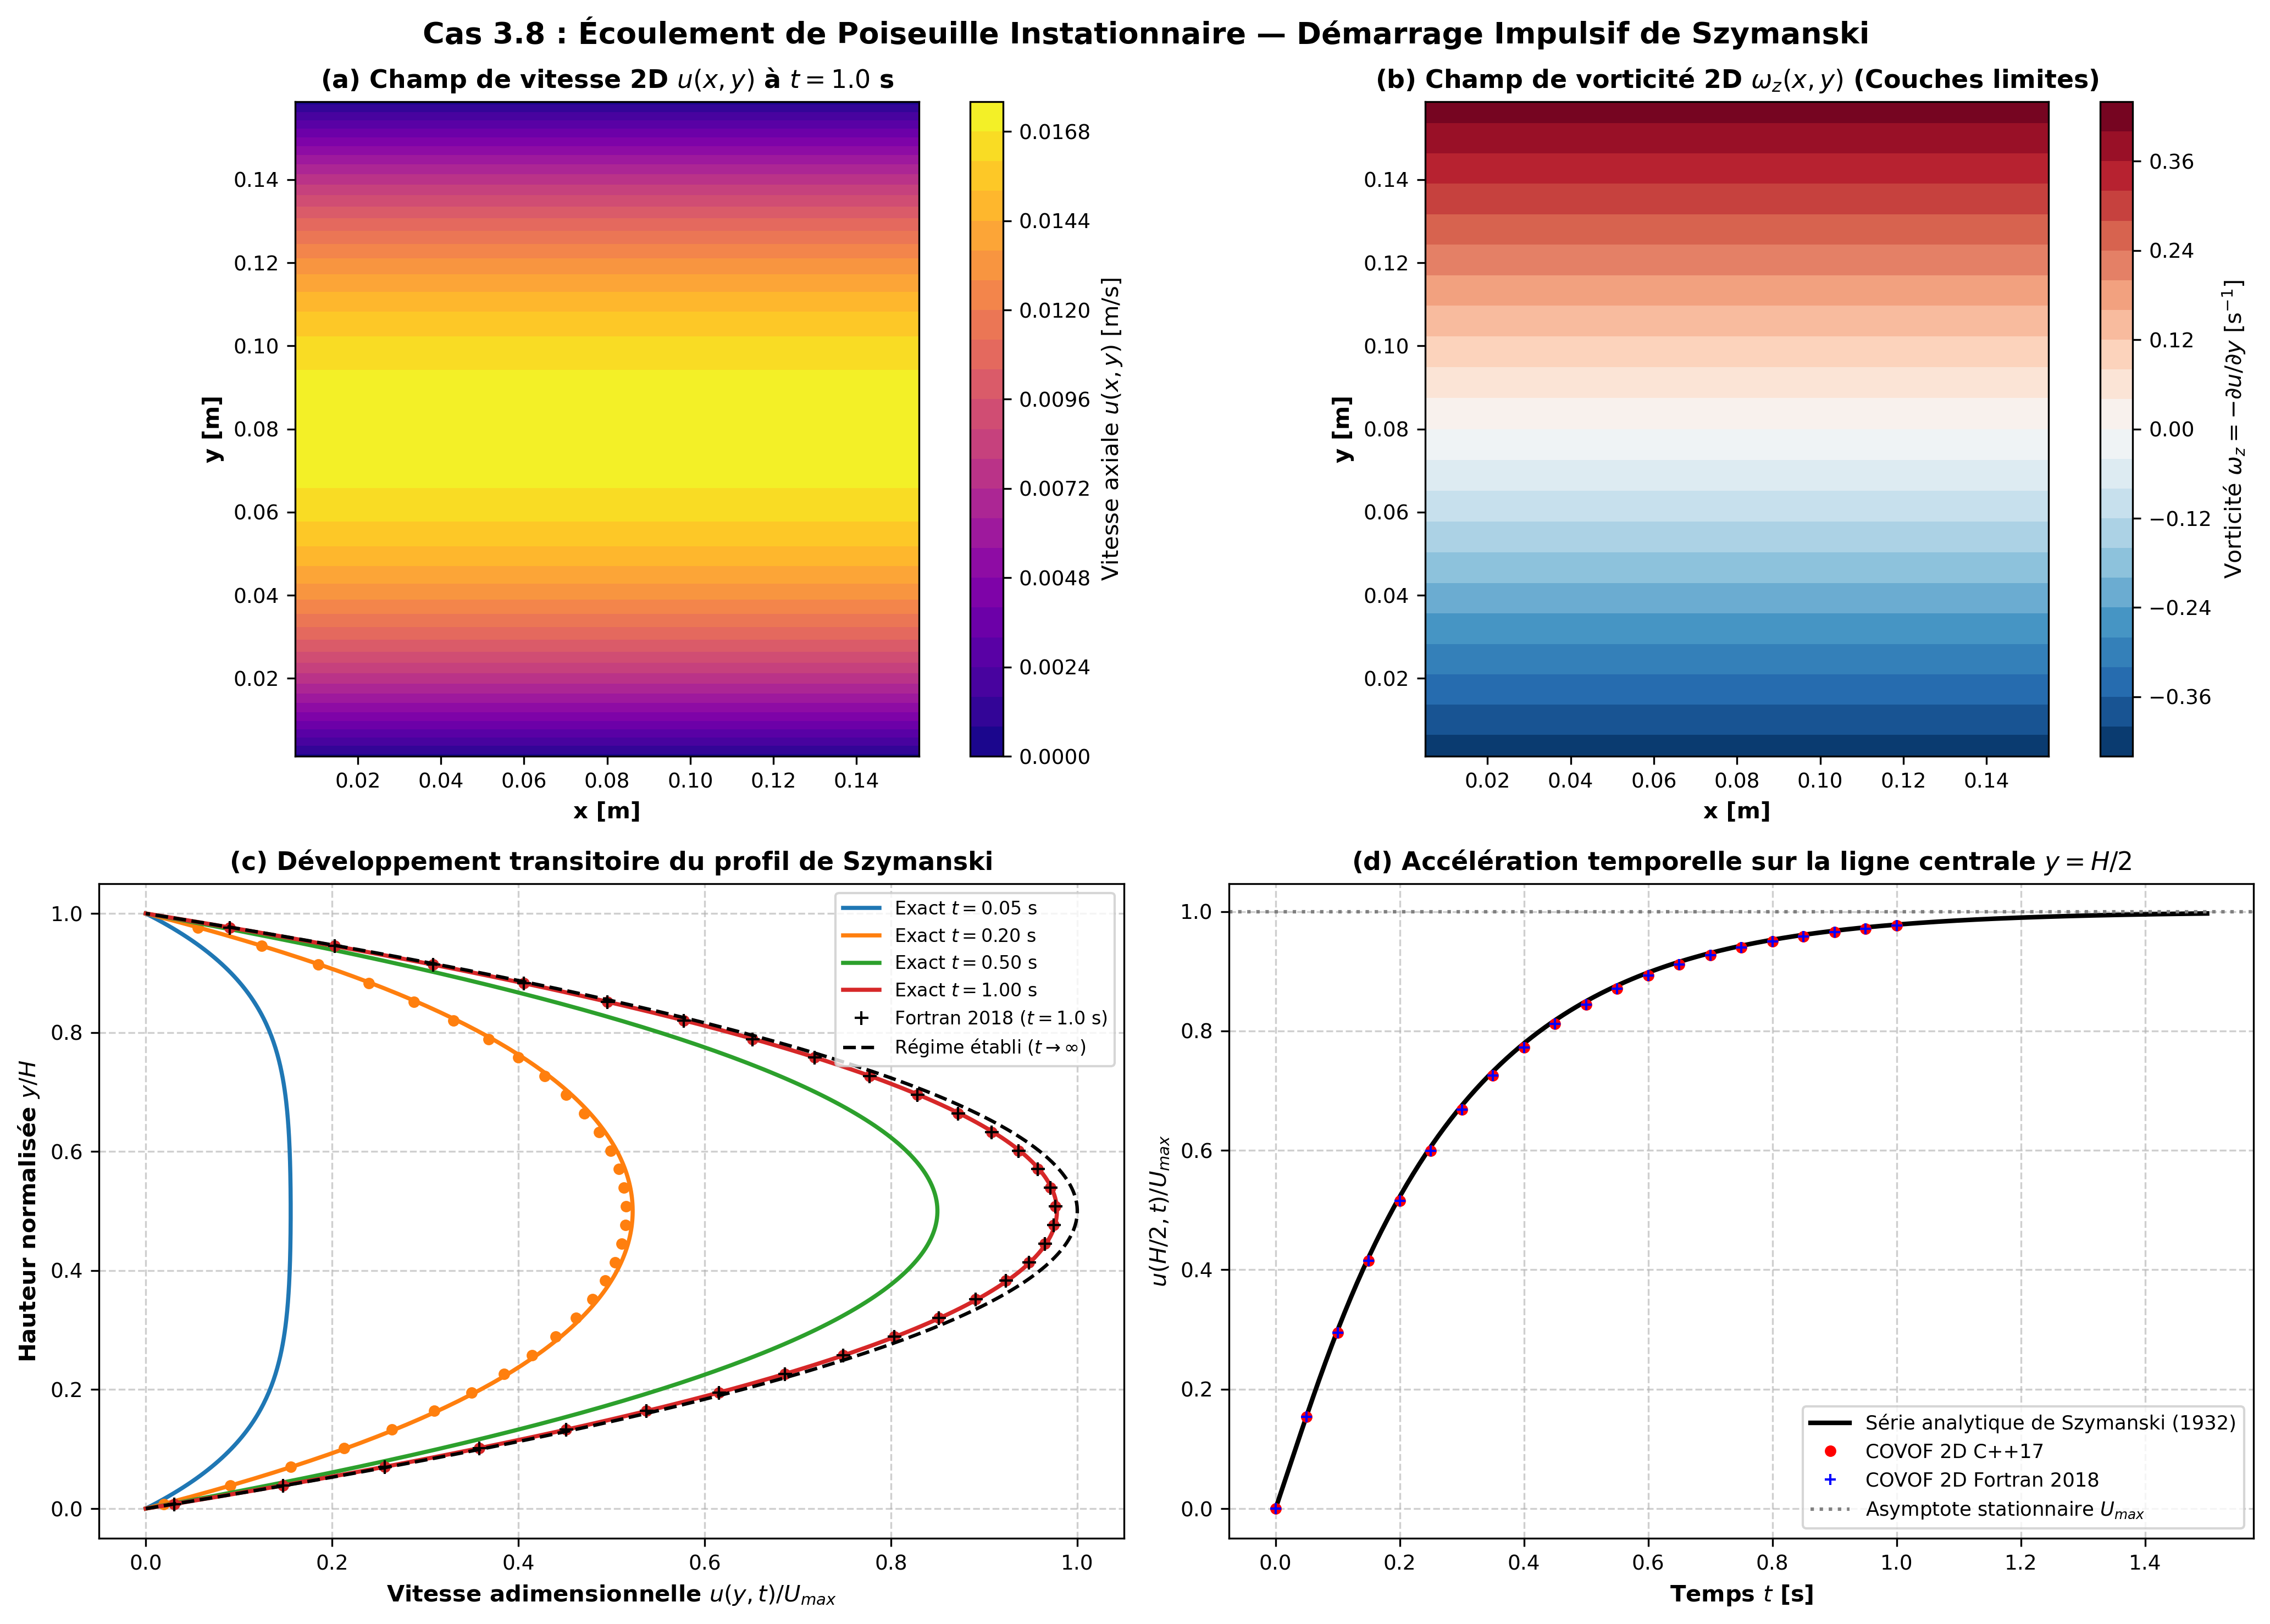
\includegraphics[keepaspectratio,alt={Szymanski Cas
3.8}]{docs/figures/fig_cas3_8_szymanski_unsteady.png}} &
\pandocbounded{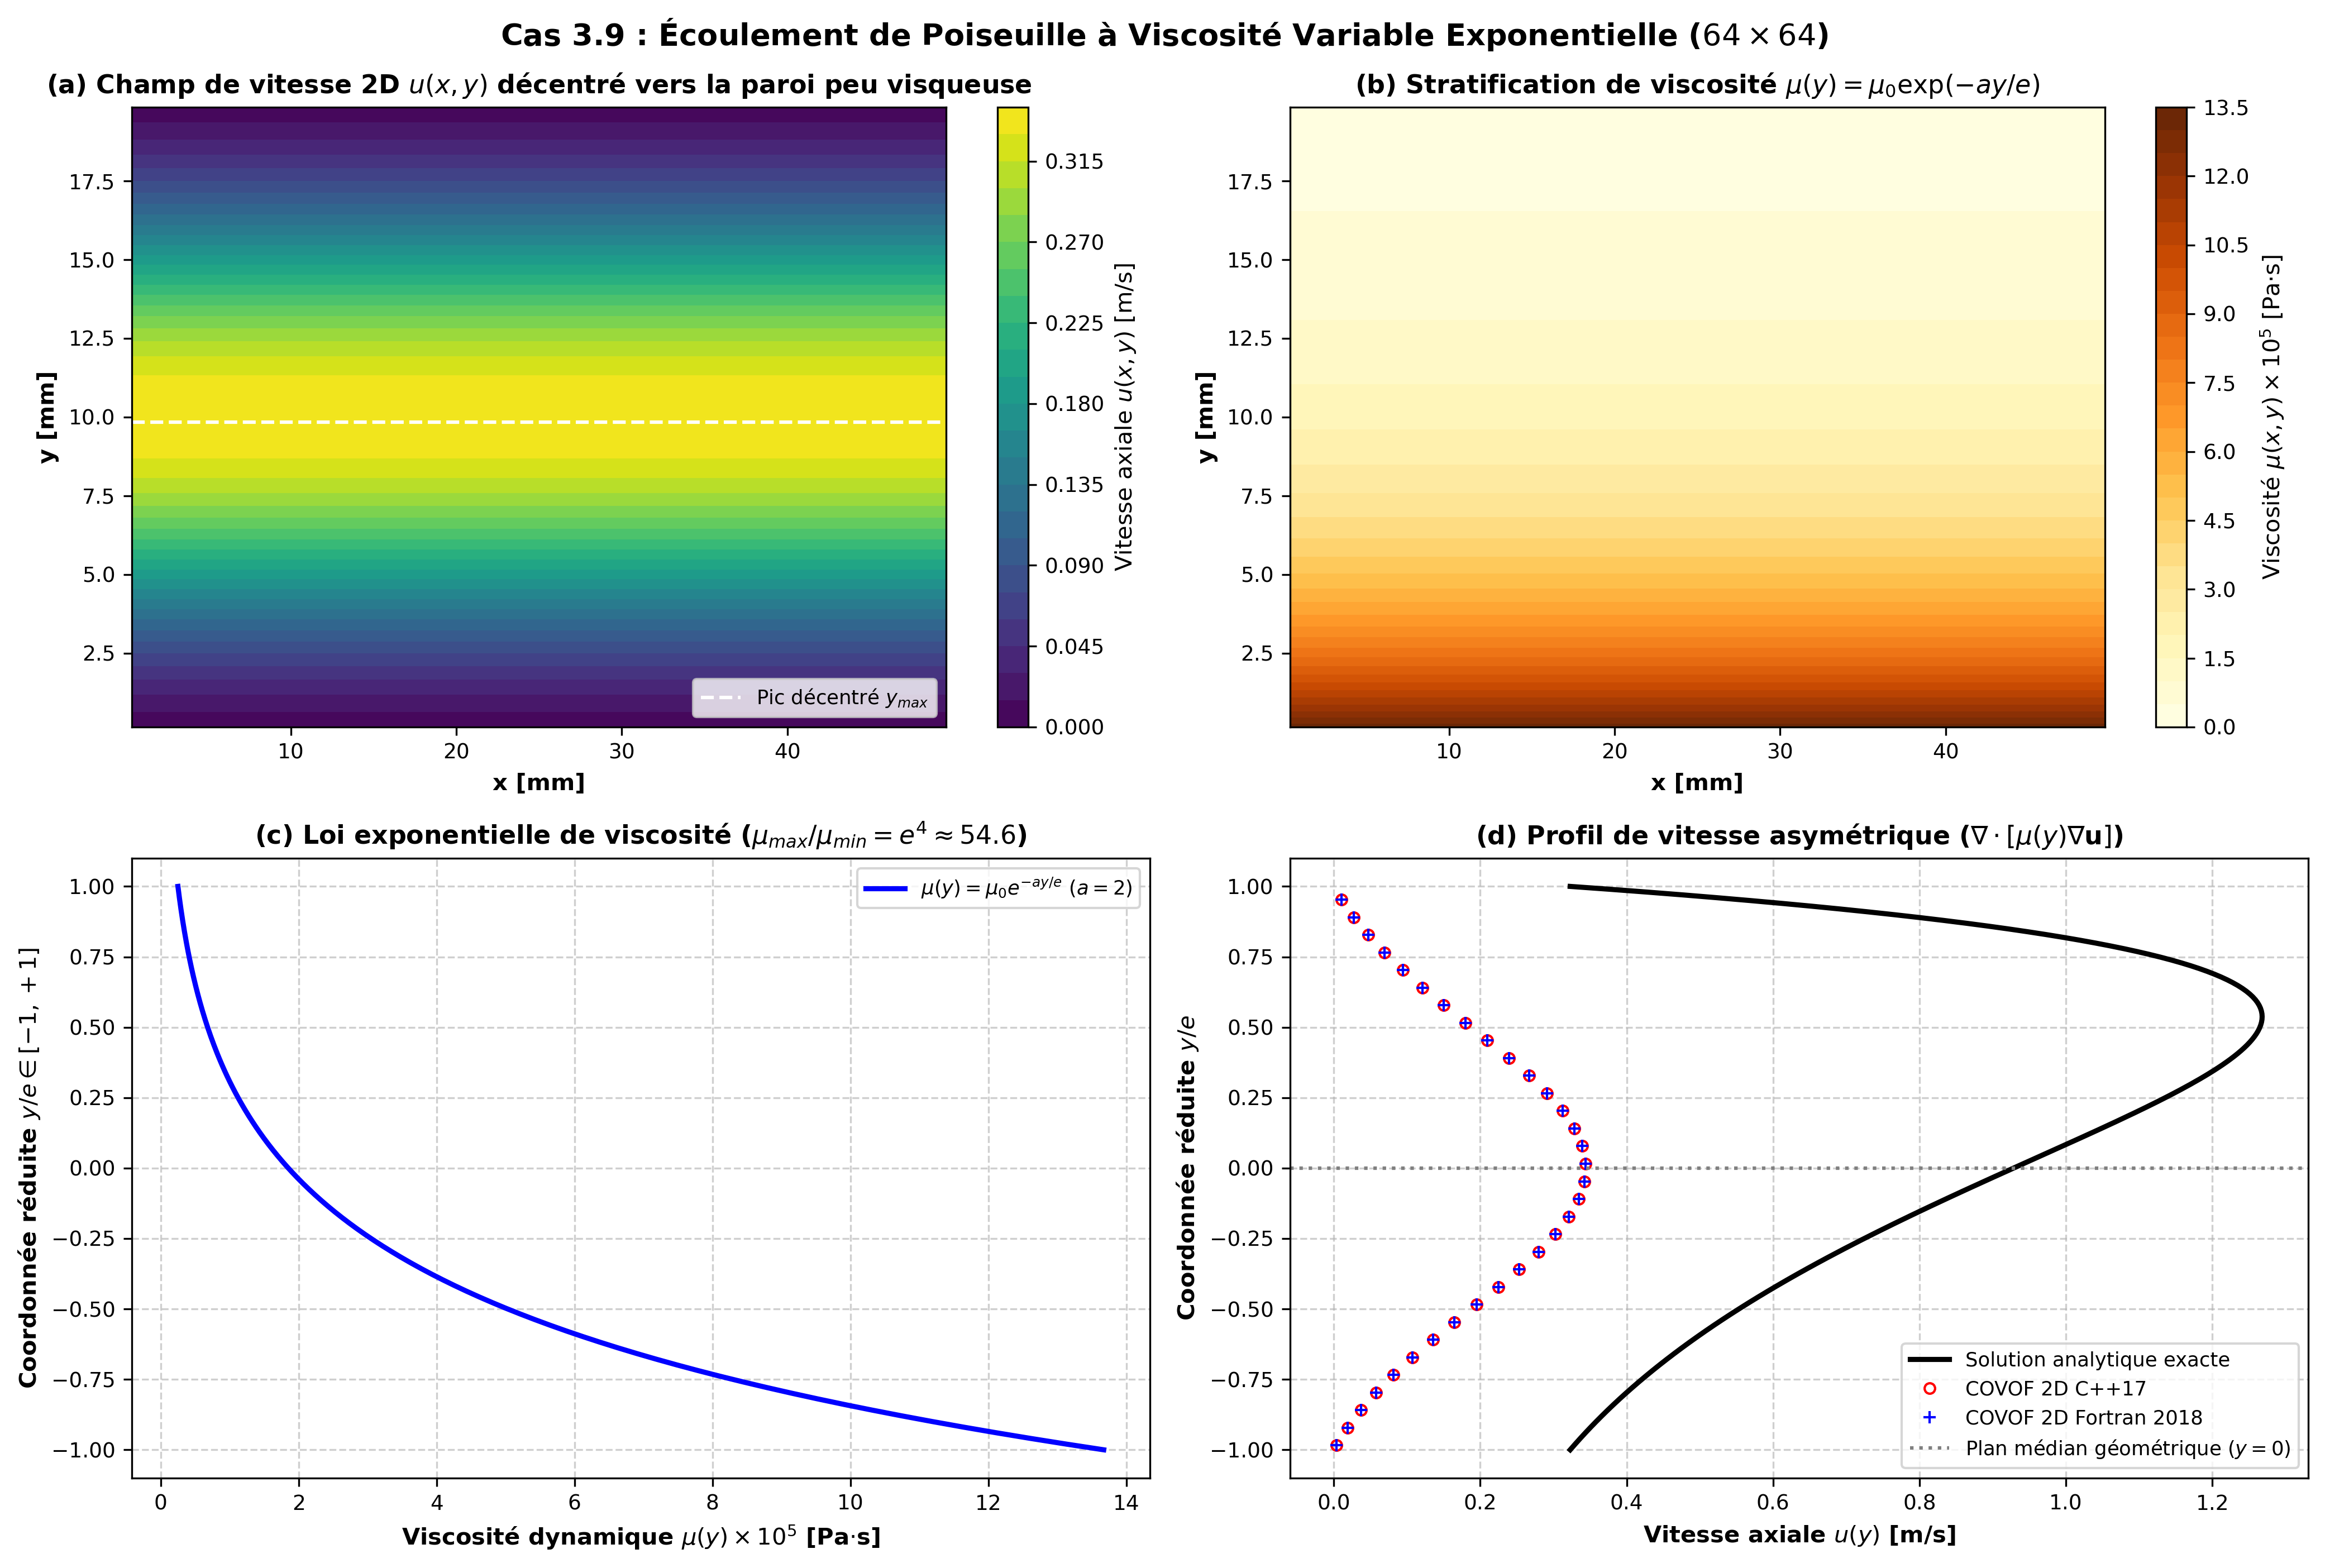
\includegraphics[keepaspectratio,alt={Viscosité Variable
Cas 3.9}]{docs/figures/fig_cas3_9_variable_viscosity.png}} \\
\emph{Concordance exacte à \(t=0.2, 0.4, 0.6, 0.8, 1.0\text{ s}\)} &
\emph{Superposition stricte avec la solution exacte
(\(u_{\max}=0.3436\text{ m/s}\))} \\
\end{longtable}
}

{\def\LTcaptype{none} % do not increment counter
\begin{longtable}[]{@{}
  >{\centering\arraybackslash}p{(\linewidth - 2\tabcolsep) * \real{0.5000}}
  >{\centering\arraybackslash}p{(\linewidth - 2\tabcolsep) * \real{0.5000}}@{}}
\toprule\noalign{}
\begin{minipage}[b]{\linewidth}\centering
Cas 4.1 : Marche Descendante d'Armaly (\(Re=100\))
\end{minipage} & \begin{minipage}[b]{\linewidth}\centering
Cas 4.5 : Lignes de Courant Cavité (\(Re=1000\))
\end{minipage} \\
\midrule\noalign{}
\endhead
\bottomrule\noalign{}
\endlastfoot
\pandocbounded{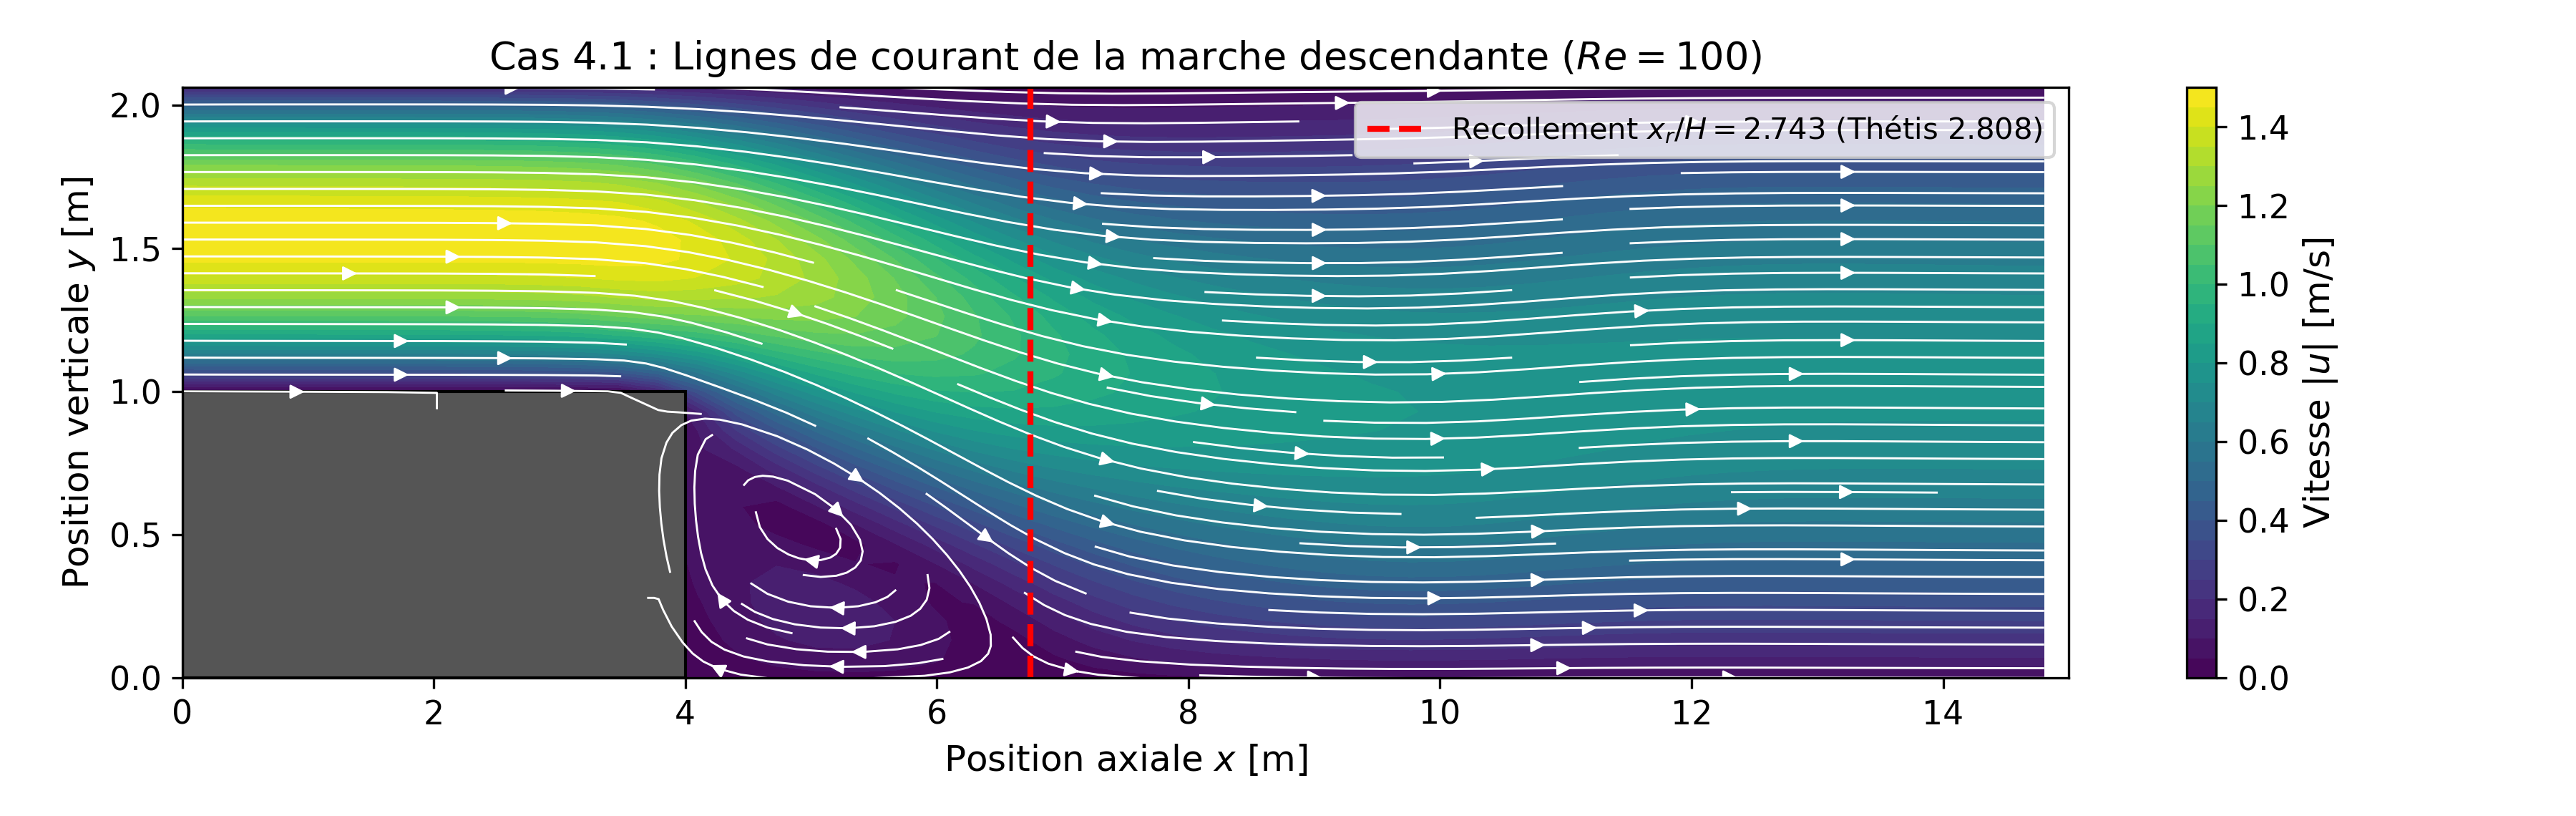
\includegraphics[keepaspectratio,alt={Marche Cas
4.1}]{docs/figures/fig_cas4_1_step_recirculation.png}} &
\pandocbounded{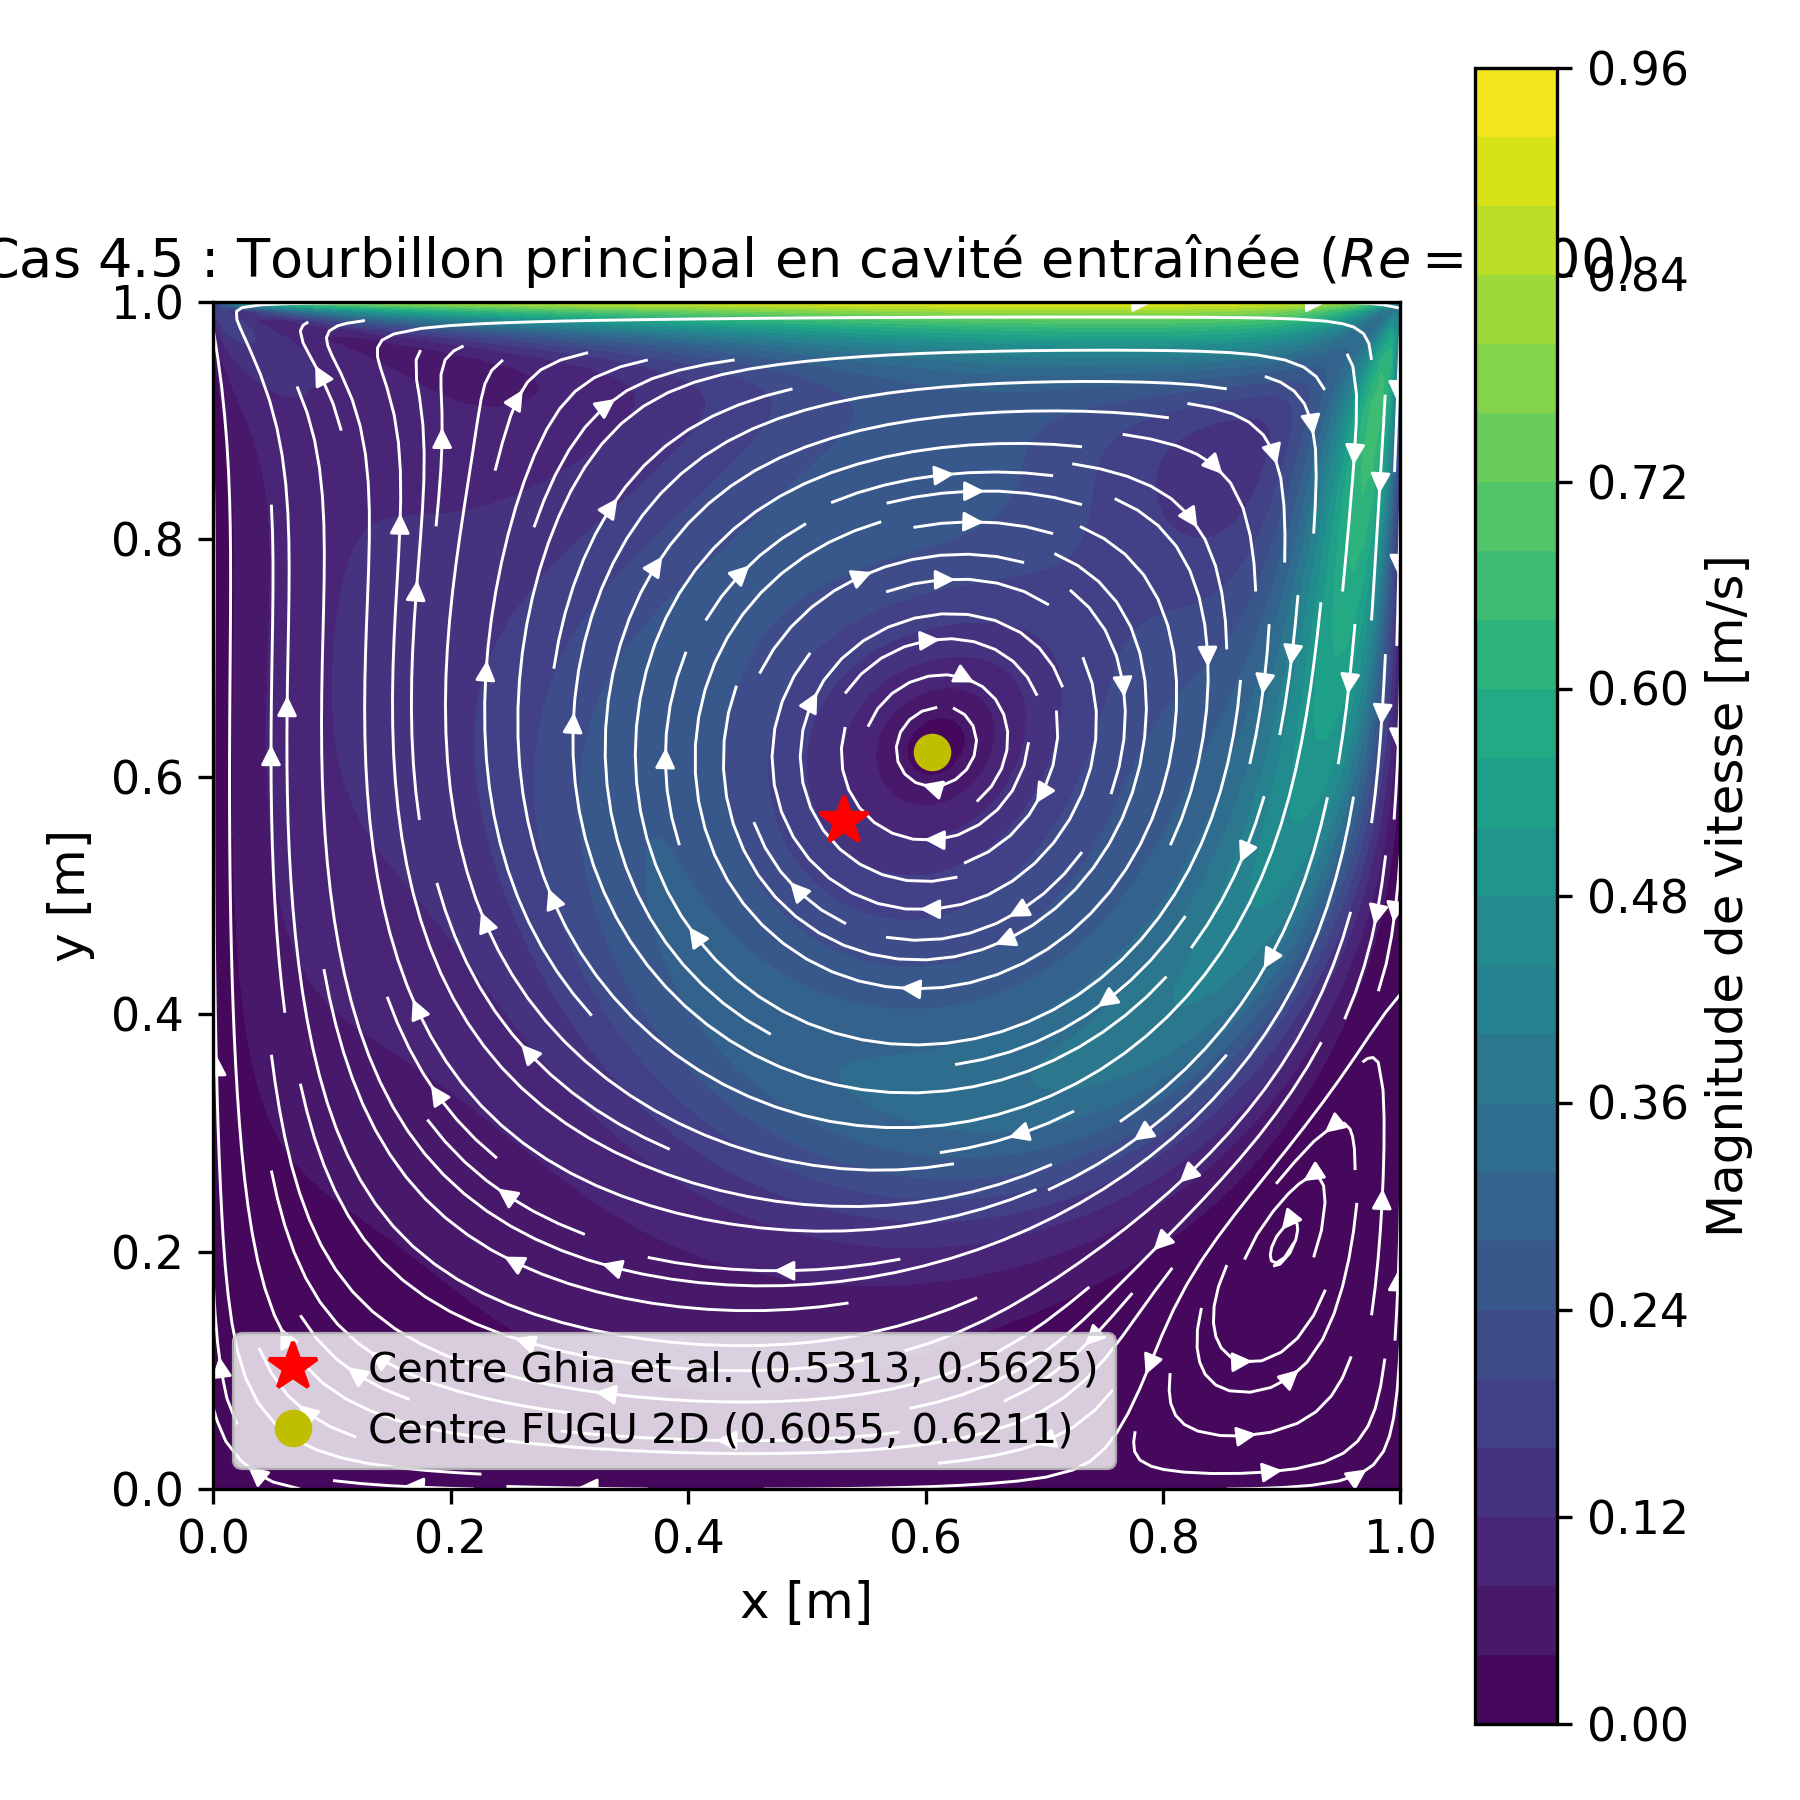
\includegraphics[keepaspectratio,alt={Cavité Cas
4.5}]{docs/figures/fig_cas4_5_cavity_streamlines.png}} \\
\emph{Recirculation primaire avec recollement à \(x_r/H = 2.72\)} &
\emph{Vortex primaire central et tourbillons secondaires de coin} \\
\end{longtable}
}

{\def\LTcaptype{none} % do not increment counter
\begin{longtable}[]{@{}
  >{\centering\arraybackslash}p{(\linewidth - 2\tabcolsep) * \real{0.5000}}
  >{\centering\arraybackslash}p{(\linewidth - 2\tabcolsep) * \real{0.5000}}@{}}
\toprule\noalign{}
\begin{minipage}[b]{\linewidth}\centering
Cas 6.1 : Convection Naturelle (\(Ra=10^4\))
\end{minipage} & \begin{minipage}[b]{\linewidth}\centering
Cas 7.4 : Saut de Pression de Laplace (Goutte)
\end{minipage} \\
\midrule\noalign{}
\endhead
\bottomrule\noalign{}
\endlastfoot
\pandocbounded{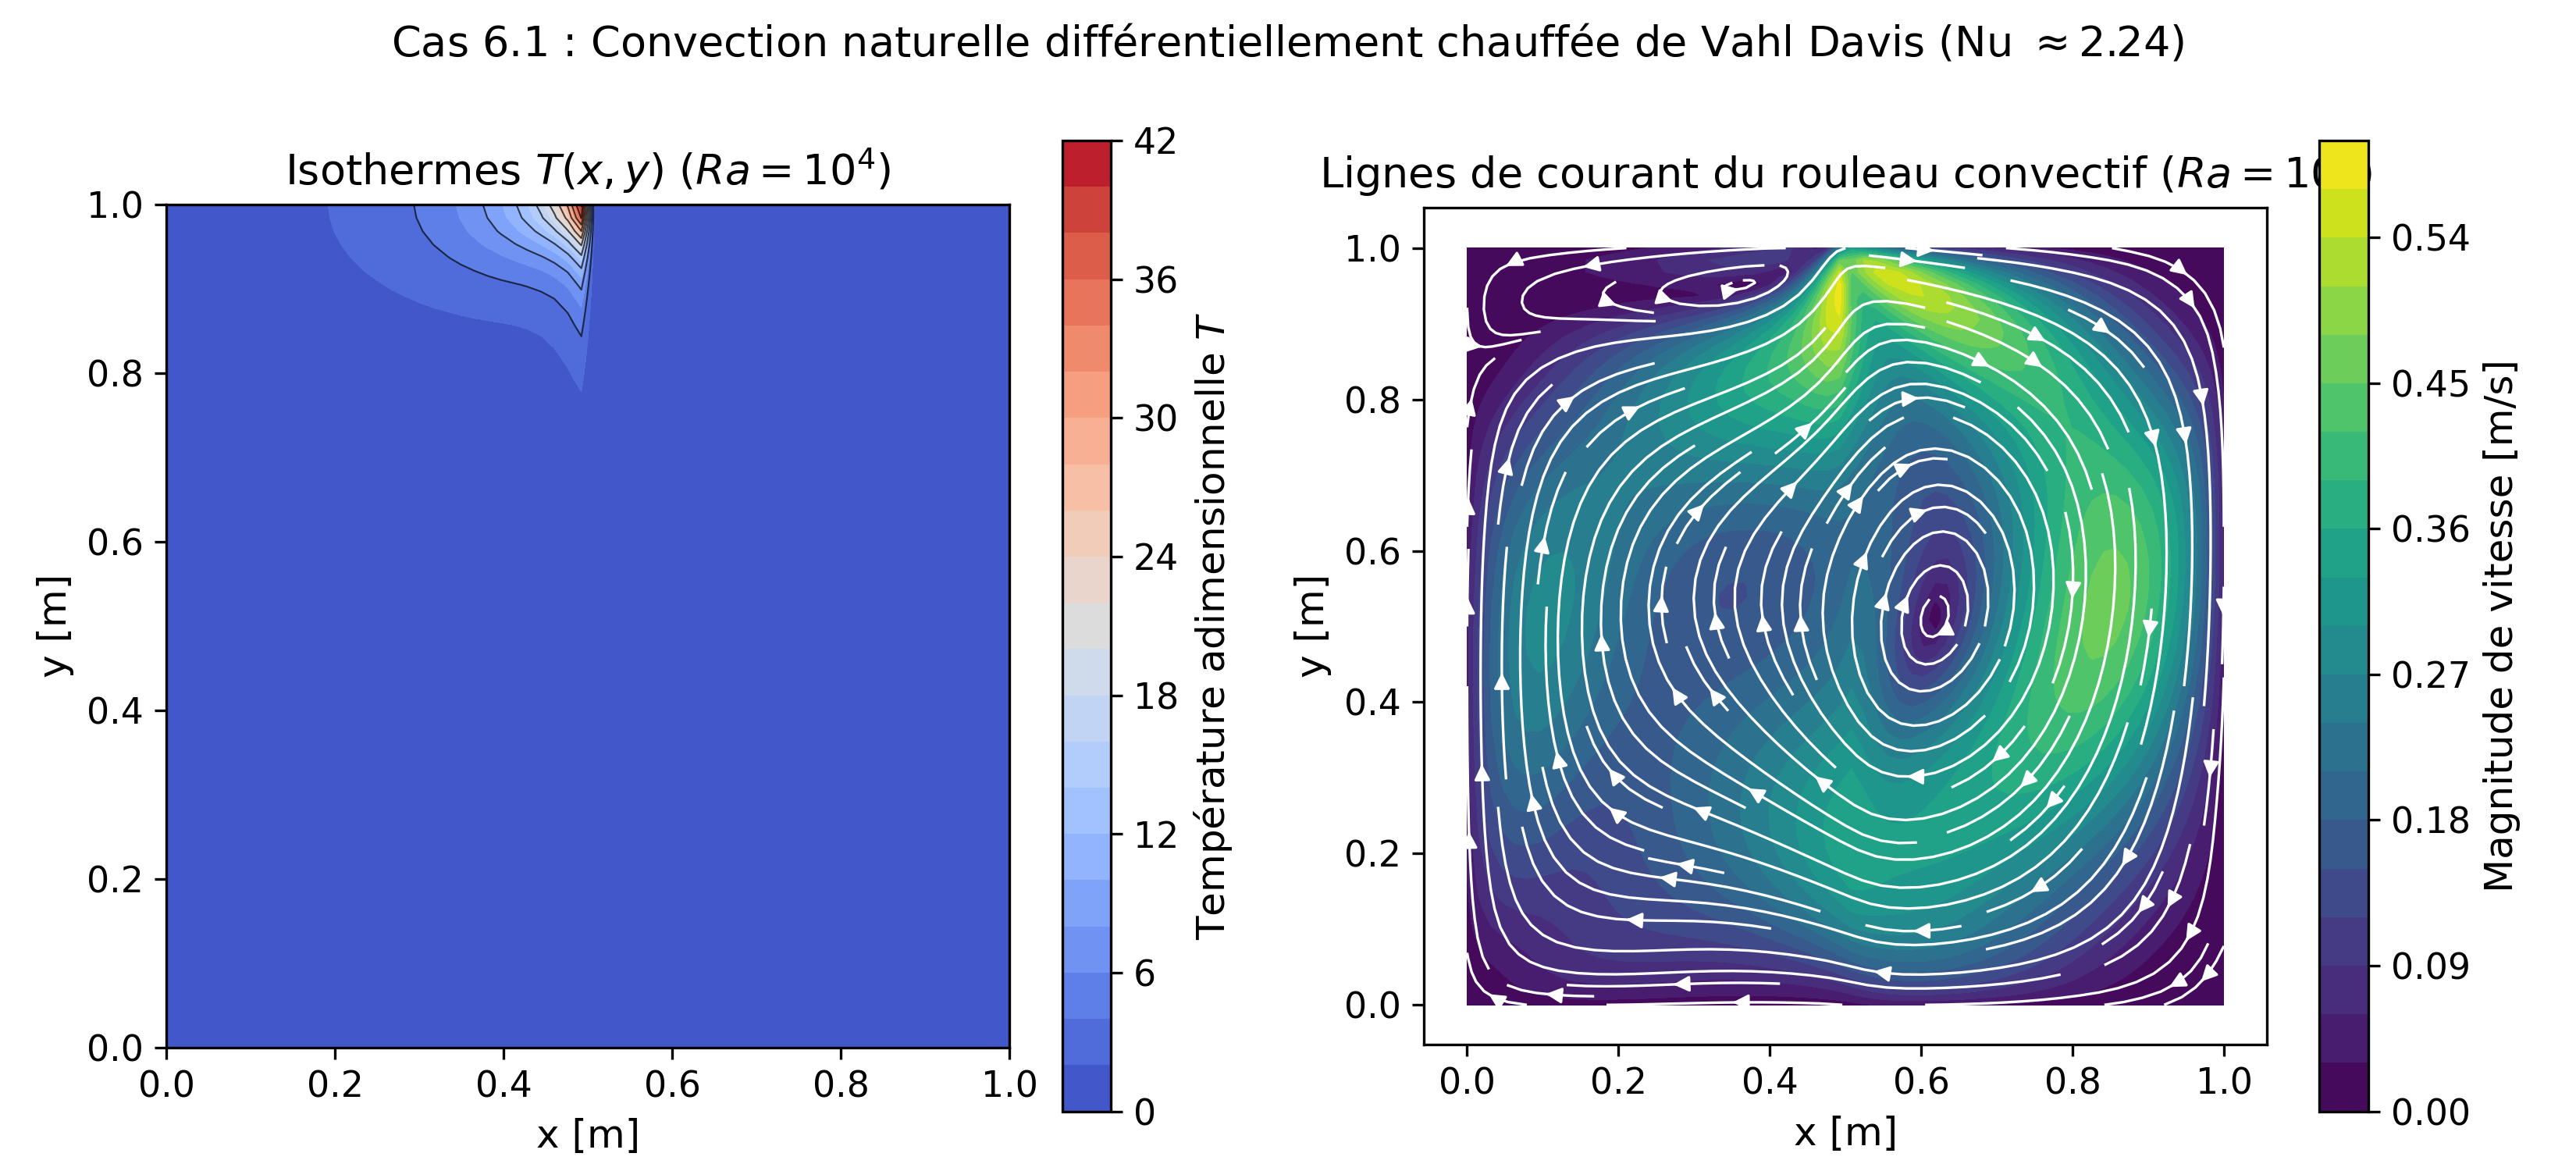
\includegraphics[keepaspectratio,alt={Convection Cas
6.1}]{docs/figures/fig_cas6_1_natural_convection.png}} &
\pandocbounded{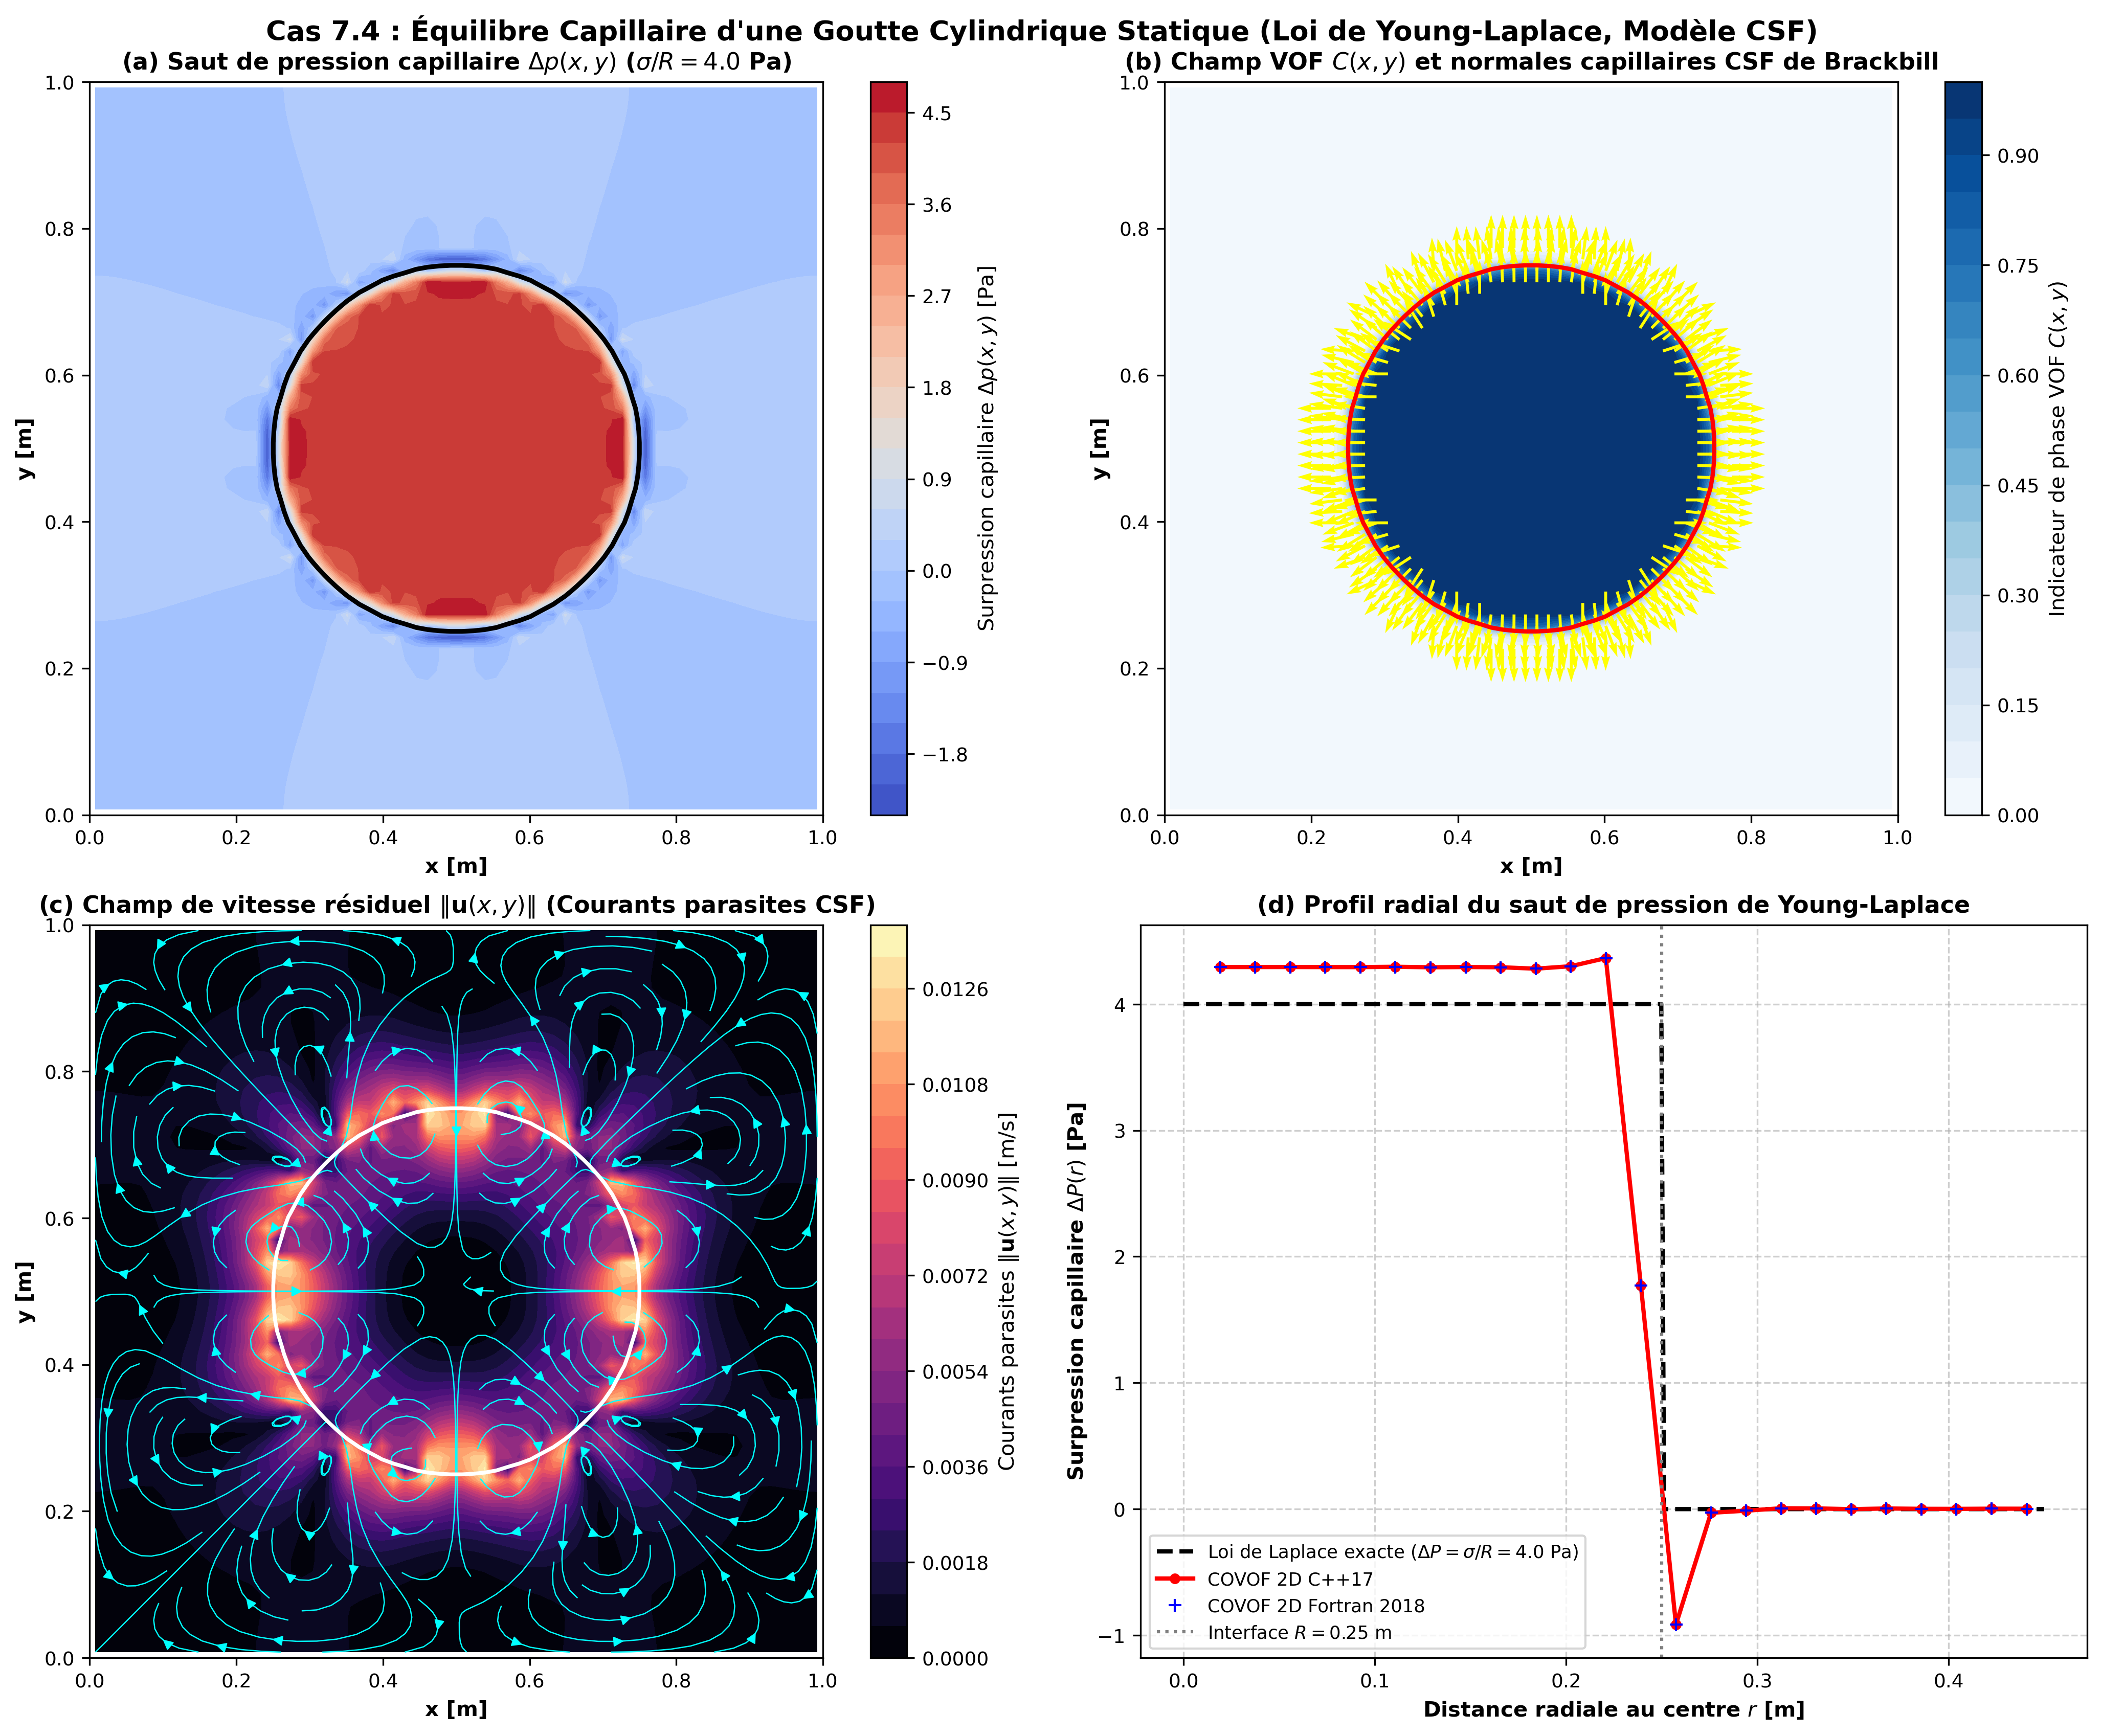
\includegraphics[keepaspectratio,alt={Goutte Laplace Cas
7.4}]{docs/figures/fig_cas7_4_laplace_droplet.png}} \\
\emph{Isothermes et rouleau convectif (\(\overline{Nu} = 2.73\))} &
\emph{Profil radial de pression
\(\Delta P = \sigma / R = 4.0\text{ Pa}\)} \\
\end{longtable}
}

\begin{center}\rule{0.5\linewidth}{0.5pt}\end{center}

\subsection{🛠 Prérequis et
Dépendances}\label{pruxe9requis-et-duxe9pendances}

\subsubsection{Environnement Logiciel}\label{environnement-logiciel}

\begin{itemize}
\tightlist
\item
  \textbf{Compilateur C++} : GCC 9+ ou Clang 11+ supportant le standard
  \textbf{C++17}.
\item
  \textbf{Bibliothèque MPI} : OpenMPI 4.0+ ou MPICH 3.3+.
\item
  \textbf{Système de Build} : CMake 3.16+ et GNU Make / Ninja.
\item
  \textbf{Environnement Python (Optionnel pour post-traitement)} :
  Python 3.8+ avec \texttt{numpy}, \texttt{matplotlib}, \texttt{pandas}.
\item
  \textbf{Visualisation 3D} : \href{https://www.paraview.org/}{ParaView}
  (support natif des fichiers multi-blocs \texttt{.pvtr}).
\end{itemize}

\subsubsection{Installation des
Prérequis}\label{installation-des-pruxe9requis}

\begin{itemize}
\item
  \textbf{macOS (Homebrew)} :

\begin{Shaded}
\begin{Highlighting}[]
\ExtensionTok{brew}\NormalTok{ install cmake open{-}mpi gcc}
\end{Highlighting}
\end{Shaded}
\item
  \textbf{Ubuntu / Debian} :

\begin{Shaded}
\begin{Highlighting}[]
\FunctionTok{sudo}\NormalTok{ apt{-}get update}
\FunctionTok{sudo}\NormalTok{ apt{-}get install }\AttributeTok{{-}y}\NormalTok{ build{-}essential cmake libopenmpi{-}dev openmpi{-}bin}
\end{Highlighting}
\end{Shaded}
\end{itemize}

\begin{center}\rule{0.5\linewidth}{0.5pt}\end{center}

\subsection{📦 Compilation et Installation
Rapide}\label{compilation-et-installation-rapide}

\begin{Shaded}
\begin{Highlighting}[]
\CommentTok{\# 1. Cloner le dépôt}
\FunctionTok{git}\NormalTok{ clone https://github.com/EL{-}I{-}Thiam/covof2d.git}
\BuiltInTok{cd}\NormalTok{ covof2d}

\CommentTok{\# 2. Configurer et compiler avec CMake}
\FunctionTok{cmake} \AttributeTok{{-}B}\NormalTok{ build }\AttributeTok{{-}DCMAKE\_BUILD\_TYPE}\OperatorTok{=}\NormalTok{Release}
\FunctionTok{cmake} \AttributeTok{{-}{-}build}\NormalTok{ build }\AttributeTok{{-}j4}

\CommentTok{\# 3. Vérifier que l\textquotesingle{}exécutable est produit dans bin/}
\FunctionTok{ls} \AttributeTok{{-}lh}\NormalTok{ bin/covof2d}
\end{Highlighting}
\end{Shaded}

\begin{center}\rule{0.5\linewidth}{0.5pt}\end{center}

\subsection{⚡ Guide d'Exécution
Rapide}\label{guide-dexuxe9cution-rapide}

\subsubsection{1. Lancer une simulation
individuelle}\label{lancer-une-simulation-individuelle}

Pour exécuter un cas test avec \(N\) processus MPI :

\begin{Shaded}
\begin{Highlighting}[]
\CommentTok{\# Cavité entraînée Re=1000 sur 4 coeurs}
\ExtensionTok{mpirun} \AttributeTok{{-}np}\NormalTok{ 4 bin/covof2d cases/cavity\_re1000.json}

\CommentTok{\# Écoulement autour d\textquotesingle{}un cylindre Re=20 sur 2 coeurs}
\ExtensionTok{mpirun} \AttributeTok{{-}np}\NormalTok{ 2 bin/covof2d cases/obstacle\_cylinder\_re20.json}

\CommentTok{\# Rupture de barrage diphasique VOF sur 4 coeurs}
\ExtensionTok{mpirun} \AttributeTok{{-}np}\NormalTok{ 4 bin/covof2d cases/dam\_break.json}
\end{Highlighting}
\end{Shaded}

\subsubsection{2. Exécuter l'ensemble de la suite de validation (13
cas)}\label{exuxe9cuter-lensemble-de-la-suite-de-validation-13-cas}

Le script automatisé
\href{scripts/run_all_benchmarks.sh}{\texttt{scripts/run\_all\_benchmarks.sh}}
compile, exécute les 13 cas tests, calcule les erreurs et affiche le
tableau récapitulatif complet :

\begin{Shaded}
\begin{Highlighting}[]
\ExtensionTok{./scripts/run\_all\_benchmarks.sh}\NormalTok{ 2}
\end{Highlighting}
\end{Shaded}

\subsubsection{3. Vérifier les métriques et générer les
figures}\label{vuxe9rifier-les-muxe9triques-et-guxe9nuxe9rer-les-figures}

\begin{Shaded}
\begin{Highlighting}[]
\CommentTok{\# Vérification analytique et génération du rapport Markdown / CSV}
\ExtensionTok{python3}\NormalTok{ scripts/verify\_cases.py}

\CommentTok{\# Tracé des 14 figures comparatives haute résolution dans docs/figures/}
\ExtensionTok{python3}\NormalTok{ scripts/generate\_validation\_figures.py}
\end{Highlighting}
\end{Shaded}

\begin{center}\rule{0.5\linewidth}{0.5pt}\end{center}

\subsection{📁 Structure du Dépôt}\label{structure-du-duxe9puxf4t}

\begin{verbatim}
covof2d/
├── CMakeLists.txt                # Configuration de compilation CMake C++17 / MPI
├── TUTORIAL.md                   # Tutoriel exhaustif pas à pas pour COVOF 2D
├── validation_summary.csv        # Données tabulées des 13 benchmarks de validation
├── validation_summary.md         # Synthèse Markdown des métriques CFD
├── bin/                          # Exécutable binaire covof2d
├── include/fugu/                 # En-têtes C++
│   ├── Config.hpp                # Parseur JSON et structures de configuration
│   ├── Mesh.hpp                  # Topologie cartésienne et décomposition 2D
│   ├── MpiComm.hpp               # Échanges de halos et synchronisation MPI
│   ├── NavierStokesSolver.hpp    # Opérateur spatial discret, Uzawa et énergie
│   ├── InterfaceTracker.hpp      # Schéma VOF-TVD Superbee et modèle CSF
│   ├── LinearSolver.hpp          # Solveurs itératifs BiCGSTAB2, PCG, GMRES
│   ├── Preconditioner.hpp        # Préconditionneur de Jacobi et SSOR
│   ├── Simulation.hpp            # Boucle temporelle et couplage multiphysique
│   └── VTKWriter.hpp             # Exporteur de maillage rectilinéaire .pvtr/.vtr
├── src/                          # Fichiers sources d'implémentation C++
├── cases/                        # 18 cas tests paramétrés au format JSON
│   ├── poiseuille.json           # Cas 3.7 : Poiseuille plan stationnaire
│   ├── poiseuille_unsteady.json  # Cas 3.8 : Poiseuille transitoire de Szymanski
│   ├── poiseuille_variable_viscosity.json # Cas 3.9 : Viscosité exponentielle
│   ├── vortex_shear_advection.json        # Cas 3.19 : Vortex avec cisaillement
│   ├── backward_facing_step.json          # Cas 4.1 : Marche descendante d'Armaly
│   ├── obstacle_cylinder_re20.json        # Cas 4.4 : Cylindre circulaire Re=20
│   ├── cavity_re1000.json        # Cas 4.5 : Cavité entraînée Re=1000
│   ├── cavity_l_shaped.json      # Cas 4.7 : Cavité en forme de L
│   ├── natural_convection_ra1e4.json # Cas 6.1 : Convection de Vahl Davis
│   ├── dam_break.json            # Cas 7.1 : Rupture de barrage VOF
│   ├── static_droplet.json       # Cas 7.4 : Goutte statique et loi de Laplace
│   └── rising_bubble.json        # Cas 7.5 : Bulle ascendante (Hysing)
├── docs/                         # Documentation technique exhaustive (>45 pages)
│   ├── INDEX.md                  # Table des matières générale
│   ├── USER_GUIDE.md             # Manuel de référence utilisateur
│   ├── DEVELOPER_GUIDE.md        # Guide d'architecture et extension développeur
│   ├── MATHEMATICAL_THEORY.md    # Formulations théoriques et discrétisation
│   ├── VALIDATION_GUIDE.md       # Cahier de vérification conforme Référence Académique CFD
│   └── figures/                  # 14 figures de validation haute définition (PNG)
└── scripts/                      # Scripts d'automatisation Python et Bash
    ├── run_all_benchmarks.sh     # Lanceur global de tous les cas de calcul
    ├── verify_cases.py           # Analyseur de convergence et métriques d'erreur
    └── generate_validation_figures.py # Générateur des figures comparatives
\end{verbatim}

\begin{center}\rule{0.5\linewidth}{0.5pt}\end{center}

\subsection{📖 Documentation et Tutoriels
Détaillés}\label{documentation-et-tutoriels-duxe9tailluxe9s}

Pour approfondir l'utilisation et le développement du code, consultez
les manuels spécialisés :

\begin{itemize}
\tightlist
\item
  \href{TUTORIAL.md}{\textbf{Tutoriel Pratique Exhaustif
  (\texttt{TUTORIAL.md})}} : guide pas-à-pas complet pour configurer,
  exécuter, post-traiter et concevoir vos propres simulations
  numériques.
\item
  \href{docs/USER_GUIDE.md}{\textbf{Manuel Utilisateur
  (\texttt{docs/USER\_GUIDE.md})}} : syntaxe exhaustive des blocs JSON,
  gestion des pas de temps, critères de convergence.
\item
  \href{docs/DEVELOPER_GUIDE.md}{\textbf{Guide Développeur
  (\texttt{docs/DEVELOPER\_GUIDE.md})}} : conventions de style, création
  d'un nouveau préconditionneur, ajout d'une équation scalaire.
\item
  \href{docs/MATHEMATICAL_THEORY.md}{\textbf{Documentation Théorique
  (\texttt{docs/MATHEMATICAL\_THEORY.md})}} : dérivation mathématique
  des équations de Navier-Stokes, tenseur des contraintes visqueuses,
  méthode CSF et schéma VOF-TVD Superbee.
\item
  \href{docs/VALIDATION_GUIDE.md}{\textbf{Cahier de Validation
  (\texttt{docs/VALIDATION\_GUIDE.md})}} : fiches de synthèse pour les
  13 cas tests du Cahier de Validation et Vérification CFD 2D.
\end{itemize}

\begin{center}\rule{0.5\linewidth}{0.5pt}\end{center}

\subsection{👥 Auteurs et Licence}\label{auteurs-et-licence}

\begin{itemize}
\tightlist
\item
  \textbf{Auteur \& Développeur} : Elhadji Ibrahima Thiam
\item
  \textbf{Laboratoire d'Inspiration} : I2M / Laboratoire TREFLE
  (Bordeaux) --- Projet Référence Académique
\item
  \textbf{Licence} : Ce projet est distribué sous licence open-source
  MIT.
\end{itemize}

\end{document}
